\documentclass[11pt,a4paper]{article}
\usepackage[margin=2.5cm]{geometry}
\usepackage{amsmath,amssymb}
\usepackage{booktabs,tabularx}
\usepackage{enumitem}
\usepackage{graphicx}
\usepackage{float}
\usepackage{xcolor}
\usepackage[most]{tcolorbox}
\usepackage[round,authoryear]{natbib}
\usepackage[colorlinks=true,linkcolor=blue!50!black,citecolor=blue!50!black]{hyperref}

\definecolor{askbg}{HTML}{FFF1E0}
\definecolor{cardframe}{HTML}{2F6FAE}
\newcommand{\ask}[1]{\par\smallskip\noindent\colorbox{askbg}{\parbox{\dimexpr\linewidth-2\fboxsep}{\textbf{Your decisions.} #1}}\par\smallskip}
\newcolumntype{Y}{>{\raggedright\arraybackslash}X}

% One card per measure, always with the same rows in the same order.
\newtcolorbox{card}[1]{enhanced, breakable, colback=white, colframe=cardframe,
  boxrule=0.6pt, arc=2pt, left=6pt, right=6pt, top=4pt, bottom=4pt,
  title={#1}, fonttitle=\bfseries, coltitle=white}
\newcommand{\row}[1]{\par\smallskip\noindent\textbf{#1}\enspace}

% Old and new wording side by side.
\newtcolorbox{oldnew}{enhanced, breakable, colback=white, colframe=black!35,
  boxrule=0.4pt, arc=2pt, left=6pt, right=6pt, top=3pt, bottom=3pt}
\newcommand{\was}[1]{\par\noindent\textbf{Now.}\enspace{\color{black!60}#1}}
\newcommand{\becomes}[1]{\par\smallskip\noindent\textbf{Proposed.}\enspace#1}

\title{Proposal, version 4\\[2pt]\large A simple score for a run (\texttt{sec:pf:measures})}
\author{For review before anything is applied}
\date{5 October 2026}

\begin{document}
\sloppy
\maketitle

\noindent Version 3 replaced the weighted criterion $\mathcal{J}$ with four
questions. Version 4 simplifies further, following your last answers.
Traffic concentration is removed, and congestion is measured by crowding
alone. Robustness is no longer a separate term. The slow loop gets one
count of its own. Versions 2 and 3 are kept as \texttt{scoring\_proposal\_v2.pdf}
and \texttt{scoring\_proposal\_v3.pdf}. Nothing in the thesis has been
changed, and the figures are drafts.

\tableofcontents

%----------------------------------------------------------------
\section{Four principles}
\label{sec:principles}

Every measure in the score follows from these four principles. A measure
that no principle asks for is left out.

\begin{enumerate}[leftmargin=1.5em]
  \item \textbf{The score judges the whole warehouse, not each layer.}
    Each layer already has its own objective, and those objectives are
    tools for producing good behaviour. The RL reward serves the fast
    loop, and the storage objective (\texttt{eq:storageobjective}) serves
    the slow loop. The score judges what both layers achieve together.
  \item \textbf{The lifelong MAPD measure decides.} The result is mean
    service time, as in \citet{ma2017lifelong_mapf}, and it is valid only
    if the fleet keeps up with the arriving tasks.
  \item \textbf{Explanations add up to the result.} Service time splits
    exactly into three parts: waiting for an agent, travelling, and being
    blocked. A change in the result can always be traced to the part that
    moved. The only other explanation is one congestion reading.
  \item \textbf{Every measure is a count or an average, and every source
    is named.} A measure taken from a paper is used as that paper defines
    it and is not claimed as a contribution. Where the thesis adds
    something, the card says what, and only that part is the thesis's own
    responsibility.
\end{enumerate}

%----------------------------------------------------------------
\section{The score at a glance}
\label{sec:glance}

\noindent\begin{tabularx}{\linewidth}{@{}lYll@{}}
  \toprule
  & Measure & Role & Source \\
  \midrule
  1 & keeping up: throughput against arrival rate, and backlog & check & \citet{ma2017lifelong_mapf} \\
  2 & mean service time $\bar\zeta_T$ & \textbf{result} & \citet{ma2017lifelong_mapf} \\
  3 & its three parts: waiting, travel, blocked & explanation & own split \\
  4 & crowding $\bar\delta_T$ & congestion & CRAMP-style density \\
  5 & units relocated per storage update $\bar\nu_T$ & slow-loop cost & own \\
  6 & runtime per timestep $\kappa_T$ & reported & \citet{ma2017lifelong_mapf} \\
  \bottomrule
\end{tabularx}

\medskip
\noindent Every result is reported as a mean with a 95\% confidence
interval over evaluation seeds. Section~\ref{sec:robust} explains why this
replaces a separate robustness measure.

\begin{figure}[H]
  \centering
  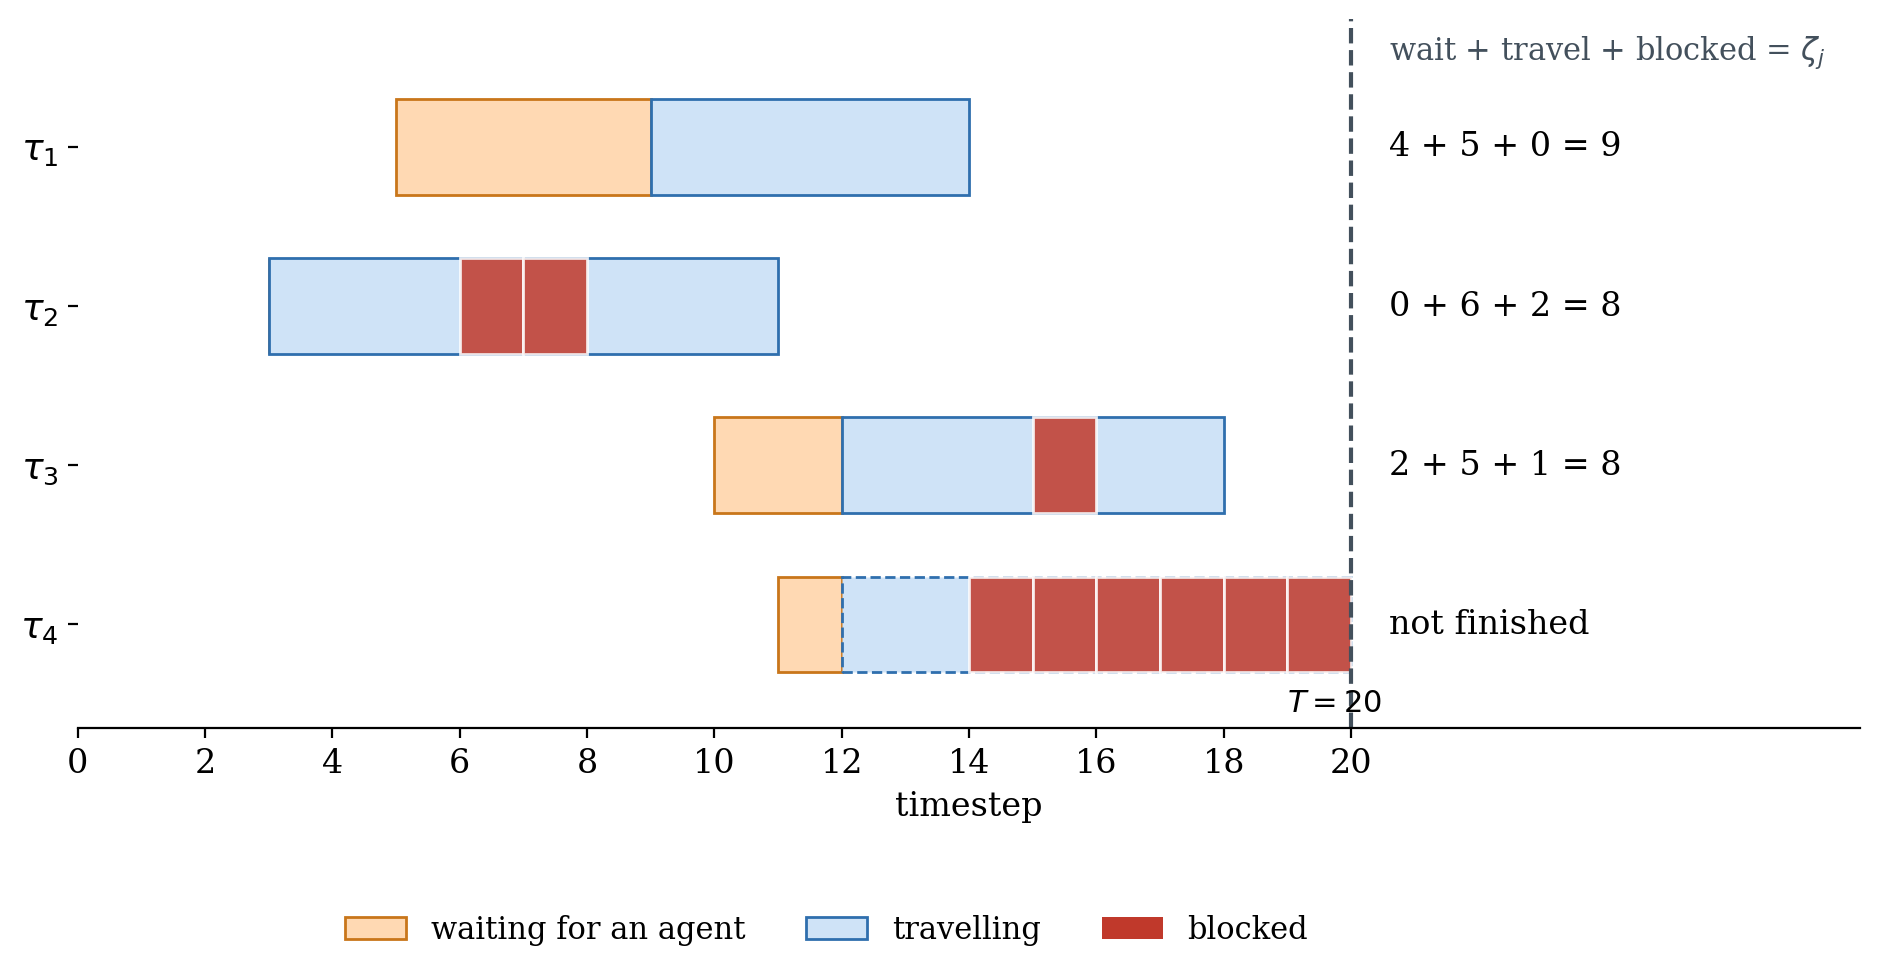
\includegraphics[width=0.9\linewidth]{timeline_split_draft.png}
  \caption{Four tasks over a horizon $T=20$, with each service time split
  into its three parts. $\tau_4$ is stuck from $t=14$ and never finishes.}
  \label{fig:timeline}
\end{figure}

\noindent Figure~\ref{fig:timeline} is the worked example for measures 1
to 3. $\tau_1$ is the task of \texttt{fig:taskroute}. Agent $a_2$ is
assigned at $t=9$ and moves one edge per timestep to D1, which it reaches
at $t=14$, so its parts are $4 + 5 + 0$.

%----------------------------------------------------------------
\section{The measures}
\label{sec:measures}

\begin{card}{1. Keeping up: throughput against arrival rate, and backlog}
\row{Question.} Is the fleet finishing tasks as fast as they arrive?

\row{What it counts.} Throughput is the number of tasks finished per
timestep. The fleet keeps up when throughput stays close to the arrival
rate. The backlog, the number of tasks released but not yet finished, is
logged at every timestep and plotted, so a run that falls behind can be
seen.

\row{Formula.}
\[
  \Lambda_T = \frac{|\mathcal{C}_T|}{T}, \qquad
  \text{the run keeps up if } \Lambda_T \ge f_{\mathrm{up}}\,\lambda_{\mathrm{task}},
  \qquad B_t = |\mathcal{Q}_t| + |\mathcal{B}_t| .
\]

\row{Worked number.} Four tasks are released and three finish within
$T = 20$. Throughput is $3/20 = 0.15$ per timestep against $4/20 = 0.20$
released, a ratio of $0.75$. The backlog ends at $B_{20} = 1$, the stuck
task $\tau_4$.

\row{Source.} \citet{ma2017lifelong_mapf} count a lifelong MAPD instance as
solved only if the service time of all tasks stays bounded, which means
the fleet keeps up. Throughput as completed tasks per unit time is the pick
rate of \citet{krnjaic2022warehouse_marl}. \emph{Own part:} the ratio test
and its threshold $f_{\mathrm{up}}$.

\row{Role.} A check, applied first. A run that does not keep up is
reported as such and is not compared on service time, because service time
only counts finished tasks. This is also how a stuck task is caught.
\end{card}

\begin{card}{2. Mean service time $\bar\zeta_T$, the result}
\row{Question.} On average, how long does a task take from its release to
its delivery?

\row{What it counts.} For each finished task, the number of timesteps from
its release to its delivery, averaged over the finished tasks.

\row{Formula.}
\[
  \bar\zeta_T = \frac{1}{|\mathcal{C}_T|}\sum_{\tau_j\in\mathcal{C}_T}\zeta_j,
  \qquad \zeta_j = t_j^{\mathrm{finish}} - t_j^{\mathrm{released}}
  \quad (\texttt{eq:servicetime}).
\]

\row{Worked number.} $\tau_1$, $\tau_2$ and $\tau_3$ take $9$, $8$ and $8$
timesteps, so $\bar\zeta_T = 25/3 \approx 8.33$.

\row{Source.} \citet{ma2017lifelong_mapf} define service time as ``the
average number of timesteps \ldots\ needed to finish executing each task
after it was added to the task set'', and use it to evaluate a MAPD
algorithm. The thesis uses it unchanged. \emph{Own part:} none.

\row{Role.} The result. Adaptive storage beats fixed storage under a
controller when both runs keep up and the confidence intervals of
$\bar\zeta_T$ do not overlap.
\end{card}

\begin{card}{3. The three parts of service time}
\row{Question.} Where did the time go?

\row{What it counts.} Every timestep of a task's life belongs to exactly
one of three parts. Before assignment the task \emph{waits for an agent}.
After assignment its agent either moves, which is \emph{travel}, or stands
still, which is \emph{blocked}. Standing still covers both a chosen wait
and a move that conflict resolution turned into a wait. The three parts
therefore always add up to the service time.

\row{Formula.} For a finished task $\tau_j$,
\[
  \zeta_j \;=\;
  \underbrace{t_j^{\mathrm{assigned}} - t_j^{\mathrm{released}}}_{\text{waiting for an agent}}
  \;+\; \underbrace{\zeta_j^{\mathrm{travel}}}_{\text{travel}}
  \;+\; \underbrace{\textstyle\sum_{t=t_j^{\mathrm{assigned}}}^{t_j^{\mathrm{finish}}-1}\omega_j(t)}_{\text{blocked}} ,
\]
with the travel part the number of moves. Each part is averaged over the
finished tasks like $\bar\zeta_T$, so the three means add up to
$\bar\zeta_T$. The blocked mean is $W_T$ of \texttt{eq:waiting}, unchanged.

\row{Worked number.} The three tasks give means of $(4+0+2)/3 = 2$
waiting, $(5+6+5)/3 \approx 5.33$ travel and $(0+2+1)/3 = 1$ blocked, which
add up to $8.33$.

\row{Source.} The service time is that of \citet{ma2017lifelong_mapf}.
\emph{Own part:} the split into three parts. It needs no new data, because
the Method already logs the assignment time and the override flag
(\texttt{sec:impl:logging}).

\row{Role.} Explains the result. Each part points to one cause.
\begin{itemize}[nosep]
  \item Waiting for an agent grows when the fleet is too small or poorly
    assigned.
  \item Travel shrinks when storage puts popular items close to where they
    are needed. This is where adaptive storage should show, so it takes
    over the role movement cost had in RQ1.
  \item Blocked time grows with congestion.
\end{itemize}
\end{card}

\begin{card}{4. Crowding $\bar\delta_T$, the congestion measure}
\row{Question.} How crowded was the space around the agents?

\row{What it counts.} Each agent's congestion feature $\delta_i(t)$, the
share of its field of view occupied by other agents, averaged over every
agent and every timestep.

\row{Formula.}
\[
  \bar\delta_T = \frac{1}{mT}\sum_{t=0}^{T-1}\sum_{i=1}^{m}\delta_i(t)
  \qquad (\delta_i(t) \text{ from \texttt{eq:congestion}}).
\]

\row{Worked number.} In the centralised panel of \texttt{fig:congestion}
(Figure~\ref{fig:congestion}), the three agents read $0$, $0.25$ and
$0.25$. Averaged, that timestep contributes $0.5/3 \approx 0.17$. Averaging
such timesteps over the horizon gives $\bar\delta_T$.

\row{Source.} The per-agent density follows CRAMP
\citep{pham2024optimizingcrowdawaremultiagentpath}, which counts the agents
in an agent's field of view and divides by the free space there. Three
differences are stated, so the thesis calls it ``CRAMP-style'' and not
CRAMP's measure.
\begin{itemize}[nosep]
  \item CRAMP uses the density only in its reward, with a threshold above
    which an area counts as crowded. It does not report the density as a
    result.
  \item CRAMP measures it over a region smaller than its field of view.
    The thesis uses the field of view $d_{\mathrm{obs}}$ itself.
  \item The thesis averages it into one reported number, with no
    threshold.
\end{itemize}
\emph{Own part:} the averaging into an outcome.

\row{Role.} The congestion measure, and the answer to RQ3. Crowding and
blocked time are read together. Crowding with no blocking costs nothing,
as with a convoy that never stops. Crowding together with blocking is
congestion that costs time.
\end{card}

\begin{figure}[H]
  \centering
  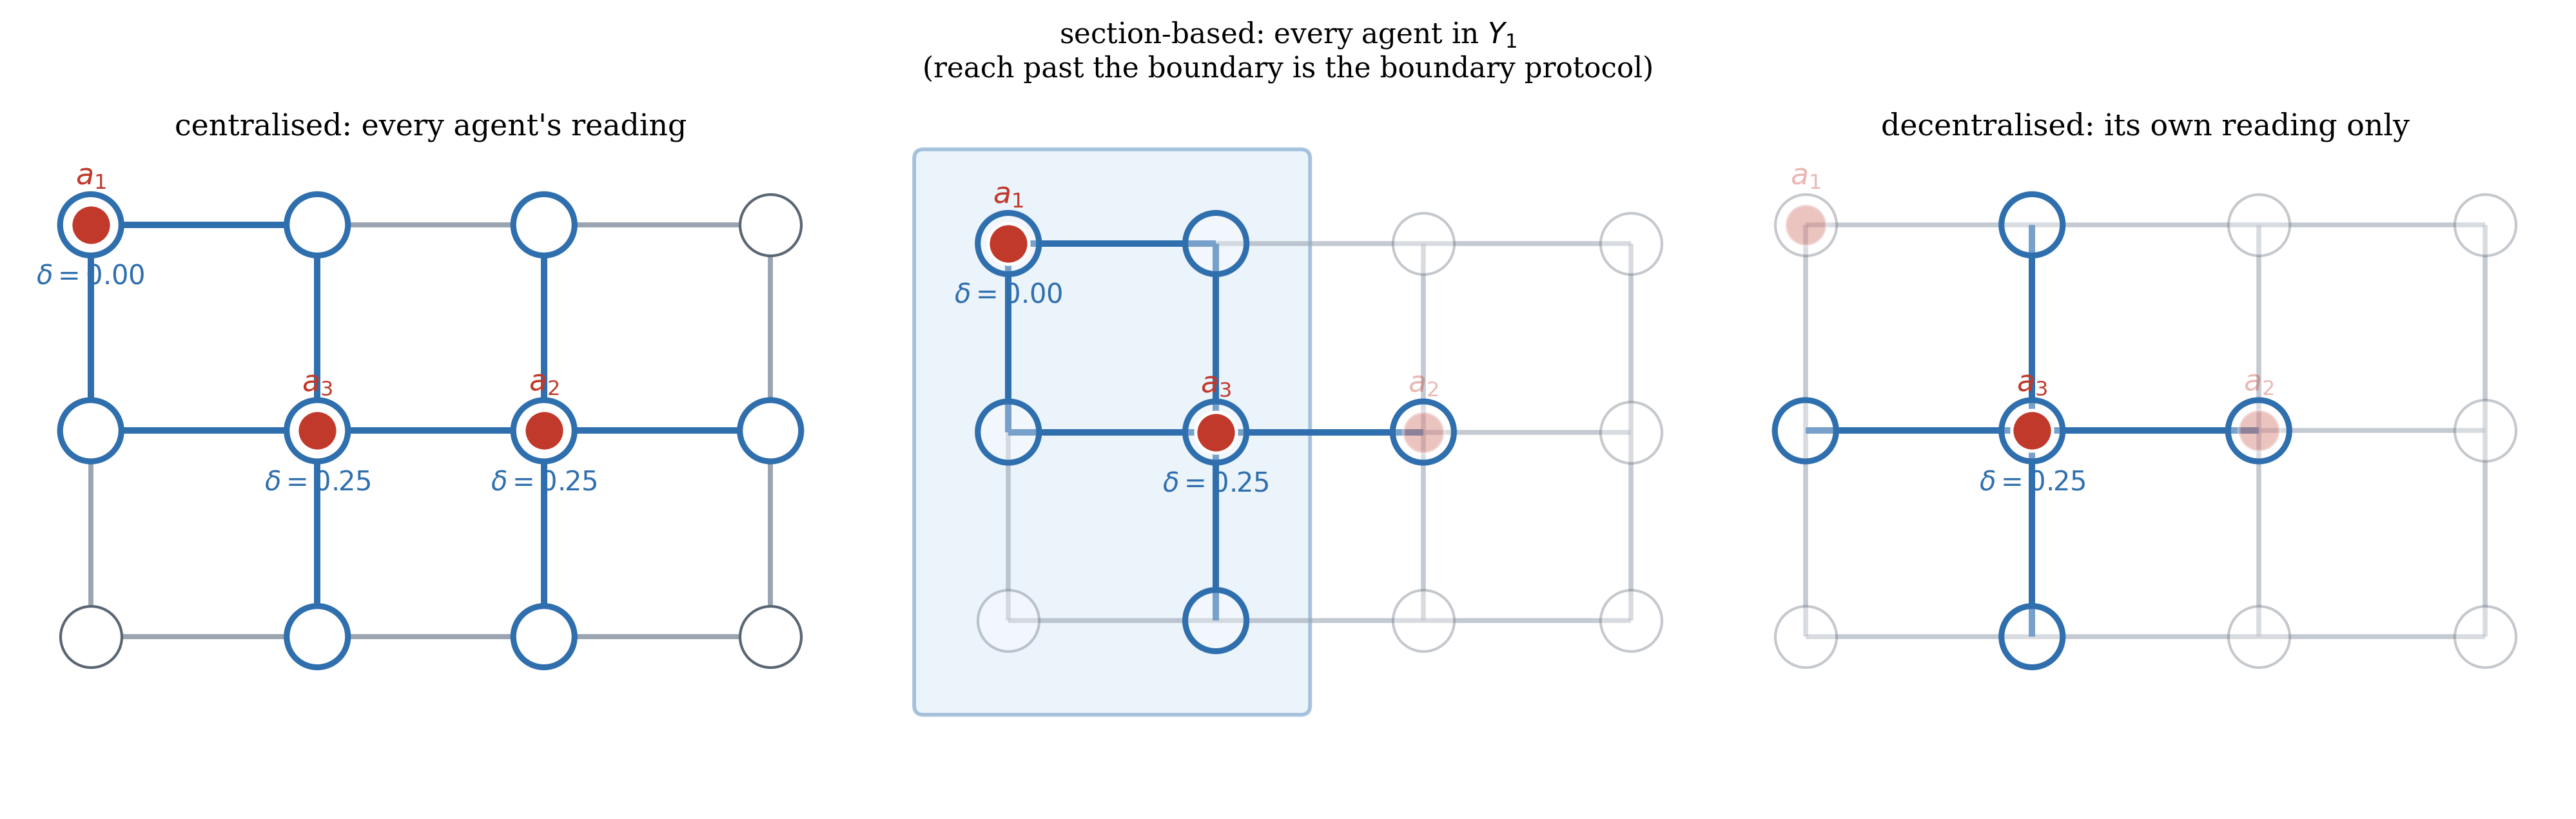
\includegraphics[width=0.95\linewidth]{congestion_mini.png}
  \caption{The existing \texttt{fig:congestion}, used for the worked number
  of the crowding measure.}
  \label{fig:congestion}
\end{figure}

\begin{card}{5. Units relocated per storage update $\bar\nu_T$, the slow-loop cost}
\row{Question.} How much stock does adaptive storage move?

\row{What it counts.} At every storage update, the number of item units
moved to a new location. Averaged over the updates in the horizon. Fixed
storage always scores $0$.

\row{Formula.} With $U$ storage updates in the horizon and $r_u$ the units
relocated at update $u$,
\[
  \bar\nu_T = \frac{1}{U}\sum_{u=1}^{U} r_u \;\le\; \nu ,
\]
where $\nu$ is the cap on relocations per update from the Method.

\row{Worked number.} With $\Delta = 50$ and $T = 1000$ there are $U = 20$
updates. If they move 120 units in total, $\bar\nu_T = 6$ units per
update. These values only serve the example.

\row{Source.} No paper in the folder reports relocation. \emph{Own part:}
the whole measure.

\row{Role.} Reported next to the result. Service time already shows what
adaptive storage gains. This count shows what it costs, which service time
cannot see, because the model does not simulate moving the stock.
\end{card}

\begin{card}{6. Runtime per timestep $\kappa_T$}
\row{Question.} How long does the controller take to choose the next joint
action?

\row{What it counts.} The wall-clock time of assignment and routing
together at each timestep, averaged over the horizon. How it is measured
is fixed in \texttt{sec:impl:cost}.

\row{Formula.}
\[
  \kappa_T = \frac{1}{T}\sum_{t=0}^{T-1}\kappa(t)
  \qquad (\texttt{eq:runtime}, \text{ unchanged}).
\]

\row{Worked number.} If deciding takes $2$\,ms at every timestep,
$\kappa_T = 2$\,ms.

\row{Source.} \citet{ma2017lifelong_mapf} report runtime per timestep and
ask for it to stay below one second for real-time lifelong operation.
\emph{Own part:} none.

\row{Role.} Reported. It is measured in seconds, so it is never combined
with service time.
\end{card}

%----------------------------------------------------------------
\section{Robustness, as other papers handle it}
\label{sec:robust}

None of the papers in the folder measures robustness as a quantity of its
own. They all report averages over many runs and vary the load.

\noindent\begin{tabularx}{\linewidth}{@{}lYY@{}}
  \toprule
  Paper & Runs per setting & Load varied \\
  \midrule
  \citet{ma2017lifelong_mapf} & one sequence of 500 tasks & 6 task rates, 5 fleet sizes \\
  CRAMP & average over 100 environments & 4 fleet sizes, 4 obstacle densities \\
  \citet{krnjaic2022warehouse_marl} & 95\% bootstrap confidence interval & two simulators, several layouts \\
  \citet{lau2022mapd} & 5 seeds, mean and standard error & fleet size and map size \\
  \bottomrule
\end{tabularx}
\medskip

\noindent The proposal therefore removes ``robustness'' from the main RQ
and adds no measure for it. Every result is reported as a mean with a 95\%
confidence interval over evaluation seeds, as \citet{krnjaic2022warehouse_marl}
do. Varying the load is already RQ4. A reader who wants to know whether a
gain is reliable reads it from the interval and from the load sweep.

%----------------------------------------------------------------
\section{The decision problem and the research question}
\label{sec:formal}

The decision problem becomes one sentence. Choose the storage rule and the
controller with the shortest expected service time among those that keep
up. Formally,
\[
  (F^\star,\pi^\star) \in \arg\min_{F\in\mathcal{F},\,\pi\in\Pi}
  \mathbb{E}\bigl[\bar\zeta_T(F,\pi)\bigr]
  \quad\text{subject to keeping up and the constraints of the model.}
\]
The expectation is over the order stream and the random seeds. The study
estimates it by the mean over evaluation seeds.

The thesis does not solve this problem. It compares fixed and adaptive
storage under each controller, so \texttt{eq:rqformal} reads
\[
  \mathbb{E}\bigl[\bar\zeta_T(F,\pi)\bigr] <
  \mathbb{E}\bigl[\bar\zeta_T(F_{\mathrm{fix}},\pi)\bigr]
  \quad\text{with non-overlapping confidence intervals, both runs keeping up.}
\]

%----------------------------------------------------------------
\section{Proposed wording of the research questions}
\label{sec:rq}

The research questions name measures that version 4 removes, so they must
change with it. The wording below is a proposal. The research questions are
yours to decide.

\begin{oldnew}
\was{How does closed-loop coupling between storage assignment and MAPD
control affect efficiency, congestion, traffic concentration, and
robustness in a graph-based warehouse?}
\becomes{How does closed-loop coupling between storage assignment and MAPD
control affect service time and congestion in a graph-based warehouse?}
\end{oldnew}

\begin{oldnew}
\was{RQ1. Does closed-loop storage adaptation improve service time,
throughput, or movement cost relative to fixed storage under otherwise
matched conditions?}
\becomes{RQ1. Does closed-loop storage adaptation shorten service time
relative to fixed storage under otherwise matched conditions, and which
part of service time changes?}
\end{oldnew}

\begin{oldnew}
\was{RQ2. How does the effect of coupling differ among centralised,
section-based, and decentralised controllers that share one learning
method and differ only in the information they condition on?}
\becomes{Unchanged.}
\end{oldnew}

\begin{oldnew}
\was{RQ3. Do congestion-sensitive storage and routing policies reduce
waiting and traffic concentration, and what efficiency trade-offs do they
introduce?}
\becomes{RQ3. Do congestion-sensitive storage and routing policies reduce
crowding and blocked time, and does the travel they add cost more service
time than they save?}
\end{oldnew}

\begin{oldnew}
\was{RQ4. How do these effects change as the number of agents and the task
arrival rate increase?}
\becomes{RQ4. How do these effects change as the number of agents and the
task arrival rate increase, and at what load does the fleet stop keeping
up?}
\end{oldnew}

\begin{oldnew}
\was{RQ5 (conditional), on local communication.}
\becomes{Unchanged.}
\end{oldnew}

\begin{oldnew}
\was{Contribution (iii). A controlled empirical analysis of when feedback
improves performance and when it amplifies congestion or concentrates
traffic on a small part of the warehouse.}
\becomes{Contribution (iii). A controlled empirical analysis of when
feedback shortens service time and when it increases congestion.}
\end{oldnew}

\begin{oldnew}
\was{Dependent variables. Mean service time, throughput, movement cost per
completed task, waiting caused by contention, traffic concentration,
backlog, and controller runtime.}
\becomes{Dependent variables. Whether the fleet keeps up (throughput against
arrival rate, and backlog), mean service time and its three parts
(waiting for an agent, travel, blocked), crowding, units relocated per
storage update, and controller runtime.}
\end{oldnew}

%----------------------------------------------------------------
\section{What is removed and what it touches}
\label{sec:touches}

\paragraph{Removed from the model.}
\begin{itemize}[nosep]
  \item $\mathcal{J}(F,\pi)$ (\texttt{eq:functional}) and its five weights
    $q_\bullet$.
  \item Traffic concentration: $H_T$, $C_T$, $E^{+}_T$, $p_T(e)$
    (\texttt{eq:entropy}, \texttt{eq:concentration}), the \texttt{[G8]}
    convention, and \texttt{fig:concentration}. The risk of funnelling
    traffic onto one aisle stays in the storage rule, through the
    congestion exposure term $K$ of \texttt{eq:storageobjective}, and its
    effect shows in crowding and blocked time.
  \item Movement cost $\bar c_T$ (\texttt{eq:movementcost}) as a reported
    measure. The travel part of service time takes its place, in the same
    unit as the result. The one-step cost $\hat c$ itself stays, since
    other parts of the model use it.
  \item Robustness as a term in the main RQ.
\end{itemize}

\paragraph{Added.} The split of service time, crowding $\bar\delta_T$,
the relocation count $\bar\nu_T$ and the threshold $f_{\mathrm{up}}$.
$\bar\nu_T$ uses the letter of the cap $\nu$, which it never exceeds.
$r_u$ is local to its formula and needs no row in the notation table.

\paragraph{Places in the thesis that change.}
\begin{itemize}[nosep]
  \item The scoring section, rewritten as the six measures in the card
    layout.
  \item \texttt{eq:decisionproblem} and \texttt{eq:rqformal}.
  \item The main RQ, RQ1, RQ3, RQ4, contribution (iii) and the dependent
    variables, as in Section~\ref{sec:rq}.
  \item The scope paragraph on deadlines (\texttt{[K2]}), which refers to
    $\mathcal{J}$ and \texttt{eq:functional}.
  \item The opening of the Method chapter, which names $\mathcal{J}$.
  \item The instrumentation section. $H_T$ is removed, and relocations per
    update are logged.
  \item The notation table.
  \item A new tag \texttt{[A20]} and a \texttt{GAPS.md} entry with the
    reasons above.
\end{itemize}

\paragraph{Not touched.} The RL reward, the storage rule $F$ and its
objective, and the congestion feature $\delta_i(t)$ itself.

%----------------------------------------------------------------
\section{Your decisions}

\ask{\begin{enumerate}[nosep,leftmargin=1.2em]
  \item Adopt the six measures and the four principles?
  \item Adopt the new RQ wording, or adjust it?
  \item Should the keep-up threshold $f_{\mathrm{up}}$ stay TBD in the
    Method tables, or do you have a value?
  \item Should the comparison rule be non-overlapping 95\% confidence
    intervals, as proposed, or a paired test over seeds? The paired test is
    stronger, because the order stream is identical under every storage
    rule (\texttt{sec:impl:instances}), but harder to explain.
\end{enumerate}}

\noindent Once you agree, the changes are applied as listed in
Section~\ref{sec:touches}. The figure scripts then move to
\texttt{thesis-progress/scripts/images/}, with outputs copied to both
\texttt{Images/} folders, and nothing is committed before you have read
the result.

\bibliographystyle{plainnat}
\bibliography{../thesis/references}

\end{document}
